\documentclass[UTF8]{ctexart}
\usepackage{amsmath}
\usepackage{cite}
\usepackage{comment}
\usepackage{tikz-feynman}
\usepackage{siunitx}
\usepackage{graphicx}
\usepackage{xcolor}

\sisetup{range-phrase = \text{--}, range-units = single}

\author{朝色}

\begin{document}

\section{HNL 的产生过程}

\subsection{$\pi^\pm$ 衰变}
AGN 环境中通过 $p - p$ 与 $p - \gamma$ 过程产生大量的 $\pi$ 介子。在标准模型下,这些介子主要衰变成为 $\mu$ 子和 $\mu$ 子中微子,而 HNL
的引入会使得 $\pi$ 介子有可能衰变到 HNL 粒子。
\begin{center}
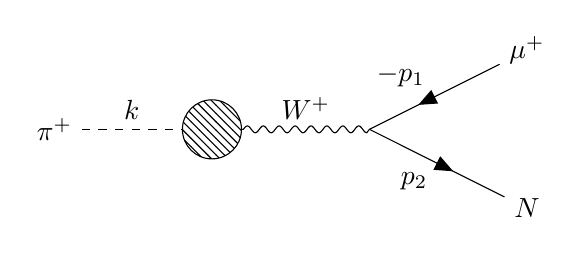
\begin{tikzpicture}
  \begin{feynman}
    \vertex [blob] (a) at (0, 0) {};
    \vertex (b) at (2, 0);
    \vertex (i1) at (-2, 0) {$\pi^+$};
    \vertex (f1) at (4, 1) {$\mu^+$};
    \vertex (f2) at (4, -1) {$N$};
    \diagram* {
      (i1) -- [scalar, edge label=$k$] (a),
      (a) -- [boson, edge label=$W^+$] (b),
      (f2) -- [anti fermion, edge label=$p_2$] (b) -- [anti fermion, edge label=$-p_1$] (f1),
    };
  \end{feynman}
\end{tikzpicture}
\end{center}
由于 HNL 粒子通过混合角 $U_{\mu N}$ 参加弱作用,$\pi^\pm$ 的衰变过程中,HNL 产生的衰变宽度与产生 $\nu_\mu$ 的宽度
只差一个混合角和运动学因子:
\begin{equation}
  \frac{\Gamma_{\pi \to \mu N}}{\Gamma_{\pi \to \mu \nu}} =
  |U_{\mu N}|^2
  \frac{((m_\mu^2 - m_N^2)^2 - m_\pi^2 (m_\mu^2 + m_N^2)) \sqrt{\lambda(m_\pi^2, m_\mu^2, m_N^2)}}{m_\mu^2 (m_\mu^2 - m_\pi^2) (m_\pi - m_\mu)}
\end{equation}
其中
\begin{equation}
  \lambda(x, y, z) = x^2 + y^2 + z^2 - 2xy - 2yz - 2zx
\end{equation}
此过程的运动学因子在 $m_N = \qtyrange{10}{30}{\mega\electronvolt}$ 的范围内从接近 1 下降到 0.7 左右,故主要的贡献在混合角,相空间抑制相比较而言不明显。

对于两体衰变,产物在质心系中的能量是固定的,能谱的分布来源于母粒子的能谱。HNL 在实验室系中的最大能量为
\begin{equation}
  \frac{E_{N,max}}{E_\pi} = \frac{m_\pi^2 - m_\mu^2 + m_N^2 + \sqrt{\lambda(m_\pi^2, m_\mu^2, m_N^2)}}{2 m_\pi^2}
\end{equation}
当取 $m_N \to 0$ 时得到无质量中微子的情况 \cite{kelner2006energy}。在 $m_N = \qtyrange{10}{30}{\mega\electronvolt}$ 的范围内,这一比值从 0.42 下
降到 0.34 左右。而对中微子这一值为 $1 - m_\mu^2 / m_\pi^2 \approx 0.43$。有质量的 HNL 相比较中微子从 $\pi$ 介子中分得较少的能量。

这同时表明对于 $\pi$ 介子衰变产生 HNL 的过程,\cite{kelner2006energy} 中对于中微子的表达式仍然适用,只需要替换上述比值即可。

\subsection{$\mu$ 子衰变}
处理 $\mu$ 子衰变这样的三体衰变会更加繁琐,但事实上,与处理 $\pi \to \mu N$ 的过程一样,新过程只是标准模型产生中微子的衰变加上混合角和不可忽略的质量。
$\mu$ 子产生 HNL 粒子的衰变过程如下:
\begin{center}
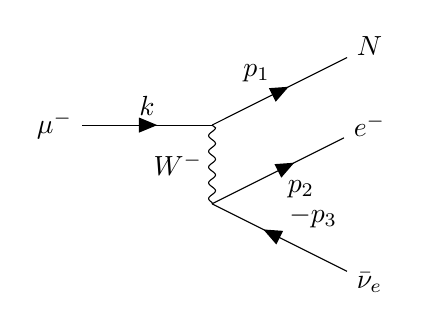
\begin{tikzpicture}
  \begin{feynman}
    \vertex (a) at (0, 0);
    \vertex (b) at (0, -1);
    \vertex (i1) at (-2, 0) {$\mu^-$};
    \vertex (f1) at (2, 1) {$N$};
    \vertex (f2) at (2, 0) {$e^-$};
    \vertex (f3) at (2, -2) {$\bar{\nu}_e$};

    \diagram* {
      (i1) -- [fermion, edge label=$k$] (a) -- [fermion, edge label=$p_1$] (f1),
      (b) -- [boson, edge label=$W^-$] (a),
      (f2) -- [anti fermion, edge label=$p_2$] (b) -- [anti fermion, edge label=$-p_3$] (f3),
    };
  \end{feynman}
\end{tikzpicture}
\end{center}
其衰变宽度具有如下平凡的形式
\begin{equation}
  \Gamma_{\mu \to N} = \Gamma_{\mu \to \nu} \times |U_{\mu N}|^2 \times \rho_\mu(m_N) 
\end{equation}
其中 HNL 的质量导致的运动学因子为
\begin{equation}
   \rho_\mu(m_N) = - r_N^8 + 8 r_N^6 + 24 r_N^4 \sinh^{-1}(\frac{r_N^{-1} - r_N}{2}) - 8 r_N^2 + 1
\end{equation}
其中 $r_N = m_N / m_\mu$。而衰变产生的 HNL 能谱为:
\begin{equation}
  \frac{d\Gamma}{dE} = \frac{G_F^2 p^2 (3 m_\mu^2 E + 3 m_N^2 E - 4 m_\mu p - 6 m_N^2 m_\mu)}{12 \pi^3 E}
\end{equation}

\begin{figure}
  \centering
  \include{wxms/spectrum_plot.tex}
  \caption{在 $\mu$ 子静止系中,其衰变产生的有质量 HNL 和无质量 $\nu_\mu$ 的能谱比较。此图中 HNL 质量
  $m_N = 20$ MeV。能谱对 $\nu_\mu$ 进行了归一化处理,并令 $|U_{\mu N}|^2 = 1$。}
  \label{fig:spec_muon_HNL}
\end{figure}

在 $\mu$ 子静止系下,我们可以比较其产生的 HNL 和 $\nu_\mu$ 的能谱(图\ref{fig:spec_muon_HNL})。$\mu$ 子产
生 HNL 的情况下,产生的 HNL 能谱形状跟 $\nu_\mu$ 较为相似,除了由于 HNL 存在质量而导致的截断。这使得相
比于 $\nu_\mu$,HNL 的能谱略向高能集中一点。

回到实验室参考系后,参考 \cite{kelner2006energy} 中的处理方式,可以得到 HNL 的能谱。这里我们忽略了 $\pi$
介子产生的 $\mu$ 子的极化问题。

\section{HNL 寿命与衰变}
\subsection{辐射衰变}
考虑圈图的情况下,HNL 可以通过风味改变中性流发生辐射衰变,直接产生 $\gamma$ 射线。典型的费曼图如下(还有另一个经由 $\mu$ 子发射光子的图):
\begin{center}
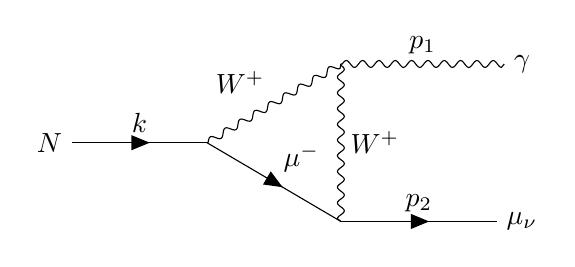
\begin{tikzpicture}
  \begin{feynman}
    \vertex (a) at (0, 0);
    \vertex (b) at (1.7, 1);
    \vertex (c) at (1.7, -1);
    \vertex (i1) at (-2, 0) {$N$};
    \vertex (f1) at (4, 1) {$\gamma$};
    \vertex (f2) at (4, -1) {$\mu_\nu$};
    \diagram* {
      (i1) -- [fermion, edge label=$k$] (a) -- [fermion, edge label=$\mu^-$] (c) -- [fermion, edge label=$p_2$] (f2),
      (a) -- [boson, edge label=$W^+$] (b) -- [boson, edge label=$W^+$] (c),
      (b) -- [boson, edge label=$p_1$] (f1),
    };
  \end{feynman}
\end{tikzpicture}
\end{center}
然而,虽然我们在本文章中只考虑 HNL 与 $\nu_\mu$ 的混合,在典型的 ISS 模型中,HNL 会与所有味的中微子混合。这意味着此过程
会受到 GIM 机制的抑制,使得衰变宽度正比于 $(\frac{m_N}{m_W})^2$,难以主导衰变过程。

如果我们考虑其它机制产生的辐射衰变,情况会有所不同。现时有很多模型可以加强这一过程,我们暂时不关注具体过程的原理,而仅关
注这一简单的两体衰变过程。



\subsection{轻子衰变}
对于 HNL 粒子的衰变过程,其必须经由与 $\nu_\mu$ 的混合完成,考虑到我们研究的质量范围,其只能通过 $Z^0$ 通道衰变。
可能的通道有:
\begin{align*}
  N & \to \nu_\mu + e^- + e^+ \\
  N & \to \nu_\mu + \nu_l + \nu_l
\end{align*}
费曼图则如下
\begin{center}
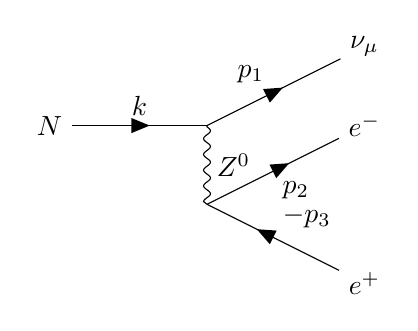
\begin{tikzpicture}
  \begin{feynman}
    \vertex (a) at (0, 0);
    \vertex (b) at (0, -1);
    \vertex (i1) at (-2, 0) {$N$};
    \vertex (f1) at (2, 1) {$\nu_\mu$};
    \vertex (f2) at (2, -0) {$e^-$};
    \vertex (f3) at (2, -2) {$e^+$};

    \diagram* {
      (i1) -- [fermion, edge label=$k$] (a) -- [fermion, edge label=$p_1$] (f1),
      (a) -- [boson, edge label=$Z^0$] (b),
      (f2) -- [anti fermion, edge label=$p_2$] (b) -- [anti fermion, edge label=$-p_3$] (f3),
    };
  \end{feynman}
\end{tikzpicture}
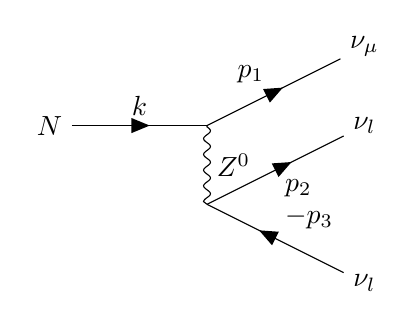
\begin{tikzpicture}
  \begin{feynman}
    \vertex (a) at (0, 0);
    \vertex (b) at (0, -1);
    \vertex (i1) at (-2, 0) {$N$};
    \vertex (f1) at (2, 1) {$\nu_\mu$};
    \vertex (f2) at (2, -0) {$\nu_l$};
    \vertex (f3) at (2, -2) {$\nu_l$};

    \diagram* {
      (i1) -- [fermion, edge label=$k$] (a) -- [fermion, edge label=$p_1$] (f1),
      (a) -- [boson, edge label=$Z^0$] (b),
      (f2) -- [anti fermion, edge label=$p_2$] (b) -- [anti fermion, edge label=$-p_3$] (f3),
    };
  \end{feynman}
\end{tikzpicture}
\end{center}
电子对衰变通道的振幅可以写为
\begin{align}
  i\mathcal{M}_{(N \to e^+ e^- \nu_\mu)} = -i\sqrt{2} U_{\mu N} G_F & [\bar{u}_e(p_2) \gamma^\mu (2 s_w^2 - \frac{1 - \gamma^5}{2}) v_e(p_3)] \\
  \times & [\bar{u}_{\nu_\mu}(p_1) \gamma_\mu (\frac{1 - \gamma^5}{2}) u_N(k)]
\end{align}
全中微子通道的振幅为
\begin{align}
  i\mathcal{M}_{(N \to \nu_l \nu_l \nu_\mu)} = -i\frac{\sqrt{2}}{2} U_{\mu N} G_F & [\bar{u}_{\nu_l}(p_2) \gamma^\mu (\frac{1 - \gamma^5}{2}) v_{\nu_l}(p_3)] \\
  \times & [\bar{u}_{\nu_\mu}(p_1) \gamma_\mu (\frac{1 - \gamma^5}{2}) u_N(k)]
\end{align}

\bibliographystyle{ieeetr}
\bibliography{ref}
\end{document}